\documentclass[a4paper]{article}

\setlength{\parskip}{0.1em}
\usepackage{caratula}
\usepackage[utf8]{inputenc}
\usepackage[T1]{fontenc}
\usepackage[spanish,es-tabla]{babel}
\usepackage{amsmath}
\usepackage{mathtools}
\usepackage{csquotes}
\usepackage{IEEEtrantools}
\usepackage{amssymb}
\usepackage{amsfonts}
\usepackage{fancyhdr}
\usepackage{pdfpages}
\usepackage{listings}
\usepackage{algorithm}
\usepackage{algpseudocode}
\usepackage{xcolor}
\usepackage{float}
\usepackage{inputenc}
\usepackage[margin=0.8in]{geometry}

\lstset { %
    language=C++,
    backgroundcolor=\color{white}, % set backgroundcolor
    basicstyle=\footnotesize,% basic font setting
}

\pagestyle{fancyplain}
% Encabezado
\lhead{Algortimos y Estructuras de Datos III}

\begin{document}
% **************************************************************************
%
%  Package 'caratula', version 0.5.1 (para componer caratulas de TPs del DC).
%  Rev (25/02/2017): Pequeño cambio para poder usar las macros de Algo1
%  En caso de dudas, problemas o sugerencias sobre este package escribir a
%  Brian J. Cardiff (bcardif arroba gmail.com).
%  Nico Rosner (nrosner arroba dc.uba.ar).
%
% **************************************************************************

% ----- Informacion sobre el package para el sistema -----------------------

\NeedsTeXFormat{LaTeX2e}
\ProvidesPackage{caratula}[2013/08/04 v0.5 Para componer caratulas de TPs del DC]
\RequirePackage{ifthen}
\usepackage{graphicx}
\graphicspath{ {img/} }


% ----- Imprimir un mensajito al procesar un .tex que use este package -----

\typeout{Cargando package 'caratula' v0.5 (2013/08/04)}

% ----- Algunas variables --------------------------------------------------

\let\Materia\relax
\let\Submateria\relax
\let\Titulo\relax
\let\Subtitulo\relax
\let\Grupo\relax
\let\Fecha\relax
\let\Logoimagefile\relax
\newcommand{\LabelIntegrantes}{}
\newboolean{showLU}
\newboolean{showEntregas}
\newboolean{showDirectores}
\newboolean{showCoDirectores}

% ----- Comandos para que el usuario defina las variables ------------------

\def\materia#1{\def\Materia{#1}}
\def\submateria#1{\def\Submateria{#1}}
\def\titulo#1{\def\Titulo{#1}}
\def\subtitulo#1{\def\Subtitulo{#1}}
\def\grupo#1{\def\Grupo{#1}}
\def\fecha#1{\def\Fecha{#1}}
\def\logoimagefile#1{\def\Logoimagefile{#1}}

% ----- Token list para los integrantes ------------------------------------

\newtoks\intlist\intlist={}

\newtoks\intlistSinLU\intlistSinLU={}

\newcounter{integrantesCount}
\setcounter{integrantesCount}{0}
\newtoks\intTabNombre\intTabNombre={}
\newtoks\intTabLU\intTabLU={}
\newtoks\intTabEmail\intTabEmail={}

\newcounter{directoresCount}
\setcounter{directoresCount}{0}
\newtoks\direcTabNombre\direcTabNombre={}
\newtoks\direcTabEmail\direcTabEmail={}

\newcounter{coDirectoresCount}
\setcounter{coDirectoresCount}{0}
\newtoks\codirecTabNombre\codirecTabNombre={}
\newtoks\codirecTabEmail\codirecTabEmail={}


% ----- Comando para que el usuario agregue integrantes --------------------

\def\integrante#1#2#3{%
    \intlist=\expandafter{\the\intlist\rule{0pt}{1.2em}#1&#2&\tt #3\\[0.2em]}%
    \intlistSinLU=\expandafter{\the\intlistSinLU\rule{0pt}{1.2em}#1 & \tt #3\\[0.2em]}%
    %
    \ifthenelse{\value{integrantesCount} > 0}{%
        \intTabNombre=\expandafter{\the\intTabNombre & #1}%
        \intTabLU=\expandafter{\the\intTabLU & #2}%
        \intTabEmail=\expandafter{\the\intTabEmail & \tt #3}%
    }{
        \intTabNombre=\expandafter{\the\intTabNombre #1}%
        \intTabLU=\expandafter{\the\intTabLU #2}%
        \intTabEmail=\expandafter{\the\intTabEmail \tt #3}%
    }%
    \addtocounter{integrantesCount}{1}%
}

\def\director#1#2{%
    \ifthenelse{\value{directoresCount} > 0}{%
        \direcTabNombre=\expandafter{\the\direcTabNombre & #1}%
        \direcTabEmail=\expandafter{\the\direcTabEmail & \tt #2}%
    }{
        \direcTabNombre=\expandafter{\the\direcTabNombre #1}%
        \direcTabEmail=\expandafter{\the\direcTabEmail \tt #2}%
    }%
    \addtocounter{directoresCount}{1}%
}

\def\codirector#1#2{%
    \ifthenelse{\value{coDirectoresCount} > 0}{%
        \codirecTabNombre=\expandafter{\the\codirecTabNombre & #1}%
        \codirecTabEmail=\expandafter{\the\codirecTabEmail & \tt #2}%
    }{
        \codirecTabNombre=\expandafter{\the\codirecTabNombre #1}%
        \codirecTabEmail=\expandafter{\the\codirecTabEmail \tt #2}%
    }%
    \addtocounter{coDirectoresCount}{1}%
}


% ----- Macro para generar la tabla de integrantes -------------------------

\newcommand{\tablaIntegrantes}{\ }

\newcommand{\tablaIntegrantesVertical}{%
\ifthenelse{\boolean{showLU}}{%
    \begin{tabular}[t]{| l @{\hspace{4ex}} c @{\hspace{4ex}} l|}
        \hline
        \multicolumn{1}{|c}{\rule{0pt}{1.2em} \LabelIntegrantes} & LU &  \multicolumn{1}{c|}{Correo electr\'onico} \\[0.2em]
        \hline \hline
        \the\intlist
        \hline
    \end{tabular}
}{
    \begin{tabular}[t]{| l @{\hspace{4ex}} @{\hspace{4ex}} l|}
        \hline
        \multicolumn{1}{|c}{\rule{0pt}{1.2em} \LabelIntegrantes} &  \multicolumn{1}{c|}{Correo electr\'onico} \\[0.2em]
        \hline \hline
        \the\intlistSinLU
        \hline
    \end{tabular}
    }%
}

\newcommand{\tablaIntegrantesHorizontal}{%
    \begin{tabular}[t]{ *{\value{integrantesCount}}{c} }
    \the\intTabNombre \\%
\ifthenelse{\boolean{showLU}}{
    \the\intTabLU \\%
}{}
    \the\intTabEmail %
    \end{tabular}%
}

\newcommand{\tablaDirectores}{%
\ifthenelse{\boolean{showDirectores}}{%
	\bigskip
	Directores

	\smallskip
    \begin{tabular}[t]{ *{\value{directoresCount}}{c} }
    \the\direcTabNombre \\%
    \the\direcTabEmail %
    \end{tabular}%
}{}%
}

\newcommand{\tablaCoDirectores}{%
\ifthenelse{\boolean{showCoDirectores}}{%
	\bigskip
	Co-Directores

	\smallskip
    \begin{tabular}[t]{ *{\value{coDirectoresCount}}{c} }
    \the\codirecTabNombre \\%
    \the\codirecTabEmail %
    \end{tabular}%
}{}%
}

\newcommand{\tablaEntregas}{%
\ifthenelse{\boolean{showEntregas}}{%
  \bigskip%
  \begin{tabular}[t]{|l p{3.5cm} p{1.5cm}|}%
  \hline%
  \rule{0pt}{1.2em} Instancia & Docente & Nota \\[0.2em] %
  \hline%
  \hline%
  \rule{0pt}{1.2em} Primera entrega & & \\[0.2em] %
  \hline%
  \rule{0pt}{1.2em} Segunda entrega & & \\[0.2em] %
  \hline%
  \end{tabular}%
}{}%
}

% ----- Codigo para manejo de errores --------------------------------------

\def\se{\let\ifsetuperror\iftrue}
\def\ifsetuperror{%
    \let\ifsetuperror\iffalse
    \ifx\Materia\relax\se\errhelp={Te olvidaste de proveer una \materia{}.}\fi
    \ifx\Titulo\relax\se\errhelp={Te olvidaste de proveer un \titulo{}.}\fi
    \edef\mlist{\the\intlist}\ifx\mlist\empty\se%
    \errhelp={Tenes que proveer al menos un \integrante{nombre}{lu}{email}.}\fi
    \expandafter\ifsetuperror}

\def\aftermaketitle{%
  \setcounter{page}{1}
}

% ----- \maketitletxt correspondiente a la versión v0.2.1 (texto v0.2 + fecha ) ---------

\def\maketitletxt{%
    \ifsetuperror\errmessage{Faltan datos de la caratula! Ingresar 'h' para mas informacion.}\fi
    \thispagestyle{empty}
    \begin{center}
    \vspace*{\stretch{2}}
    {\LARGE\textbf{\Materia}}\\[1em]
    \ifx\Submateria\relax\else{\Large \Submateria}\\[0.5em]\fi
    \ifx\Fecha\relax\else{\Large \Fecha}\\[0.5em]\fi
    \par\vspace{\stretch{1}}
    {\large Departamento de Computaci\'on}\\[0.5em]
    {\large Facultad de Ciencias Exactas y Naturales}\\[0.5em]
    {\large Universidad de Buenos Aires}
    \par\vspace{\stretch{3}}
    {\Large \textbf{\Titulo}}\\[0.8em]
    {\Large \Subtitulo}
    \par\vspace{\stretch{3}}
    \ifx\Grupo\relax\else\textbf{\Grupo}\par\bigskip\fi
    \tablaIntegrantes
    \end{center}
    \vspace*{\stretch{3}}
    \newpage\aftermaketitle}

% ----- \maketitletxtlogo correspondiente v0.2.1 (texto con fecha y logo) ---------

\def\maketitletxtlogo{%
    \ifsetuperror\errmessage{Faltan datos de la caratula! Ingresar 'h' para mas informacion.}\fi
    \thispagestyle{empty}
    \begin{center}
    \ifx\Logoimagefile\relax\else\includegraphics{\Logoimagefile}\fi \hfill 
\includegraphics{logo_dc.jpg}\\[1em]
    \vspace*{\stretch{2}}
    {\LARGE\textbf{\Materia}}\\[1em]
    \ifx\Submateria\relax\else{\Large \Submateria}\\[0.5em]\fi
    \ifx\Fecha\relax\else{\large \Fecha}\\[0.5em]\fi
    \par\vspace{\stretch{1}}
    {\large Departamento de Computaci\'on}\\[0.5em]
    {\large Facultad de Ciencias Exactas y Naturales}\\[0.5em]
    {\large Universidad de Buenos Aires}
    \par\vspace{\stretch{3}}
    {\Large \textbf{\Titulo}}\\[0.8em]
    {\Large \Subtitulo}
    \par\vspace{\stretch{3}}
    \ifx\Grupo\relax\else\textbf{\Grupo}\par\bigskip\fi
    \tablaIntegrantes
    \end{center}
    \vspace*{\stretch{4}}
    \newpage\aftermaketitle}

% ----- \maketitlegraf correspondiente a la versión v0.3 (gráfica) -------------

\def\maketitlegraf{%
    \ifsetuperror\errmessage{Faltan datos de la caratula! Ingresar 'h' para mas informacion.}\fi
%
    \thispagestyle{empty}

    \ifx\Logoimagefile\relax\else\includegraphics{\Logoimagefile}\fi \hfill 
\includegraphics{logo_dc.jpg}

    \vspace*{.06 \textheight}

    \noindent \textbf{\huge \Titulo}  \medskip \\
    \ifx\Subtitulo\relax\else\noindent\textbf{\large \Subtitulo} \\ \fi%
    \noindent \rule{\textwidth}{1 pt}

    {\noindent\large\Fecha \hspace*\fill \Materia} \\
    \ifx\Submateria\relax\else{\noindent \hspace*\fill \Submateria}\fi%

    \medskip%
    \begin{center}
        \ifx\Grupo\relax\else\textbf{\Grupo}\par\bigskip\fi
        \tablaIntegrantes

        \tablaDirectores

        \tablaCoDirectores

        \tablaEntregas
    \end{center}%
    \vfill%
%
    \begin{minipage}[t]{\textwidth}
        \begin{minipage}[t]{.55 \textwidth}
            
\includegraphics{logo_uba.jpg}
        \end{minipage}%%
        \begin{minipage}[b]{.45 \textwidth}
            \textbf{\textsf{Facultad de Ciencias Exactas y Naturales}} \\
            \textsf{Universidad de Buenos Aires} \\
            {\scriptsize %
            Ciudad Universitaria - (Pabell\'on I/Planta Baja) \\
                Intendente G\"uiraldes 2610 - C1428EGA \\
            Ciudad Aut\'onoma de Buenos Aires - Rep. Argentina \\
                Tel/Fax: (++54 +11) 4576-3300 \\
            http://www.exactas.uba.ar \\
            }
        \end{minipage}
    \end{minipage}%
%
    \newpage\aftermaketitle}

% ----- Reemplazamos el comando \maketitle de LaTeX con el nuestro ---------
\renewcommand{\maketitle}{\maketitlegraf}

% ----- Dependiendo de las opciones ---------
%
% opciones:
%   txt     : caratula solo texto.
%   txtlogo : caratula txt con logo del DC y del grupo (opcional).
%   graf    : (default) caratula grafica con logo del DC, UBA y del grupo (opcional).
%
\@makeother\*% some package redefined it as a letter (as color.sty)
%
% Layout general de la caratula
%
\DeclareOption{txt}{\renewcommand{\maketitle}{\maketitletxt}}
\DeclareOption{txtlogo}{\renewcommand{\maketitle}{\maketitletxtlogo}}
\DeclareOption{graf}{\renewcommand{\maketitle}{\maketitlegraf}}
%
% Etiqueta Autores o Integrantes
%
\DeclareOption{integrante}{\renewcommand{\LabelIntegrantes}{Integrante}}
\DeclareOption{autor}{\renewcommand{\LabelIntegrantes}{Autor}}
%
% Formato tabla de integrantes
%
\DeclareOption{intVert}{\renewcommand{\tablaIntegrantes}{\tablaIntegrantesVertical}}
\DeclareOption{intHoriz}{\renewcommand{\tablaIntegrantes}{\tablaIntegrantesHorizontal}}
\DeclareOption{conLU}{\setboolean{showLU}{true}}
\DeclareOption{sinLU}{\setboolean{showLU}{false}}
\DeclareOption{conEntregas}{\setboolean{showEntregas}{true}}
\DeclareOption{sinEntregas}{\setboolean{showEntregas}{false}}
\DeclareOption{showDirectores}{\setboolean{showDirectores}{true}}
\DeclareOption{hideDirectores}{\setboolean{showDirectores}{false}}
\DeclareOption{showCoDirectores}{\setboolean{showCoDirectores}{true}}
\DeclareOption{hideCoDirectores}{\setboolean{showCoDirectores}{false}}
%
% Opciones predeterminadas
%
\ExecuteOptions{intVert}%
\ExecuteOptions{graf}%
\ExecuteOptions{integrante}%
\ExecuteOptions{conLU}%
\ExecuteOptions{hideDirectores}%
\ExecuteOptions{hideCoDirectores}%
\ExecuteOptions{sinEntregas}%
%
\ProcessOptions\relax

\include{resumen}

\tableofcontents

\section{Introducción Teorica}
\label{sec:introduccion}

\section{Desarrollo}
\label{sec:desarrollo}

\subsection{Algoritmo de Fuerza Bruta}

En ciencias de la computación, la técnica de búsqueda por fuerza bruta o búsqueda exhaustiva, también conocida como generate and test (generar y probar), es una forma muy general de resolver problemas y un paradigma de algoritmos que consiste en enumerar sistemáticamente todos los posibles candidatos a ser solución y luego chequear si cada candidato satisface o no el enunciado del problema. \footnote{$https://es.wikipedia.org/wiki/B\%C3\%BAsqueda\_de\_fuerza\_bruta$}

En nuestro problema "Problema de la Mochila (Gloppi Ya)"  dado un conjunto de pedidos con un peso y beneficio asociado y una mochila de capacidad fija, la solución consiste en el subconjunto de pedidos que maximice la suma de beneficios y a su vez no supere la capacidad de la mochila.

Siguiendo nuestro paradigma de resolución, deberíamos generar todas las posibles soluciones al problema y luego chequear si satisfacen el enunciado. Para ello, generaremos todos los subconjuntos de pedidos (posibles soluciones) y luego nos quedaremos con aquel que maximice la suma de beneficios y a su vez quepa en la mochila.


\begin{algorithm}
\caption{Fuerza Bruta}\label{selection}
\begin{algorithmic}[1]
\Procedure{bruteForce}{$vector \ \ pedidos, \ int \ \ w$}
	\State $vector \ subSets$
   \For{\textbf{$i \gets 1$ to} $2^{|pedidos|}$}
   	\State $wi \gets 0$
	\State $pi \gets 0$
    \For{\textbf{$j \gets 0$ to} $|pedidos|$}
    \If{$j-esimo\ bit\ de\ i\ esta\ en\ 1$}
    	\State $wi \gets wi\ +\ pedidos[j].beneficio$
	\State $pi \gets pi\ +\ pedidos[j].peso$
	\EndIf
	\EndFor

	\If{$wi \ > \ w$}
	\State $pi \gets -1$
	\EndIf

	\State $subSets[i] \gets pi $
    \EndFor
   	\State $Return \ \ maxElement(subSets)$
\EndProcedure
\end{algorithmic}
\end{algorithm}


Al comienzo de nuestra solución propuesta hacemos un ciclo el cual ira desde $1$ hasta $2^{n}$, es decir desde 1 hasta la cantidad de subconjuntos. Dentro de este ciclo haremos otro ciclo en n, la cantidad de elementos del conjunto (véase también como la cantidad de bits de $2^{n}$), y en el cual usaremos a la variable j como un numero binario, fijándonos que bits están en 1 para tener en cuenta esas posiciones del vector pedidos (considerando ese subconjunto) para sumar su beneficio y peso (correspondientemente acumulado en las variables wi y pi) y sea una posible solución(generando de esta manera, todos los subconjuntos posibles). Finalmente nos preguntamos si la suma de los elementos considerados supera la capacidad de la mochila, de ser así seteamos su beneficio en $-1$ (eliminando la solución), caso contrario almacenamos el beneficio total en el vector subSets. Y por ultimo retornamos el elemento de mayor valor del vector subSets, siendo este el mayor beneficio obtenible.

\subsection*{Análisis de Complejidad}
Describiremos cada acción con su complejidad y luego realizaremos la suma total.


Complejidad de calcular la suma de todos los elementos de los $2^{n}$ posibles subconjuntos de pedidos que pueden llegar a ser a lo sumo de longitud n = O($n*2^{n}$).


Complejidad de algunos checkeos y comparaciones de cantidades = O(1).


Complejidad Total del algoritmo = O($n*2^{n}$).

\subsection{Backtracking}

Backtracking es una técnica algorítmica que se encarga de encontrar todas las soluciones a un problema, construyendo de a pasos los candidatos a la solución. La ventaja por sobre los algoritmos de fuerza bruta proviene de que podemos eliminar un gran número de candidatos con un único test utilizando podas. Las mismas nos permiten determinar cuándo debemos abandonar a un candidato y que no es posible que alcancen una solución del problema.

Para aplicar backtracking a nuestro problema, lo que notamos es que dado un elemento, una solución puede contenerlo o no. De esta manera, queremos construir nuestro árbol de recurrencias (o árbol de backtracking) en dónde en el paso i, o bien incluímos al i-ésimo elemento en la solución parcial o bien lo excluímos. Esto nos lleva a generar un árbol que contiene a todos los subconjuntos posibles.

El siguiente pseudocódigo muestra como podemos obtener ésto facilmente:

\begin{algorithm}
\caption{Backtracking}\label{selection}
\begin{algorithmic}[1]
\Procedure{backtracking}{$pair \ \ res, \ pair \ \ parcial, \ int \ \ indice$}
   \For{\textbf{$i \gets indice$ to} $|pedidos|$}
   	\State $parcial.w \gets parcial.w + pedidos[i].w$
	  \State $parcial.b \gets parcial.b + pedidos[i].b$
    \If{parcial es mejor que res}
    \State $res \gets parcial$
    \EndIf
    \State Backtracking(res, parcial, i+1)
    \State $parcial.w \gets parcial.w - pedidos[i].w$
	  \State $parcial.b \gets parcial.b - pedidos[i].b$

	 \EndFor
\EndProcedure
\end{algorithmic}
\end{algorithm}

Veamos bien como funciona el algoritmo. Las variables res y parcial representan a la solución final y a la solución parcial que estamos estudiando respectivamente, miesntras que índice es el elemento que tenemos que decidir si agregar o no a nuestro candidato. El llamado inicial va a tener a res y a parcial como los pares <0,0>, e índice comenzará en 0. El for recorre todos los elementos que quedan por visitar en un llamado dado (desde índice hasta el final del arreglo de pedidos). En este  ciclo, primero agregamos el elemento a nuestra solución parcial. Si ahora parcial es mejor que res, actualizamos res. Luego, realizamos el llamado recursivo aumentando el índice para recorrer los caminos que incluye al elemento i. Por último, sacamos al elemento i de parcial y continuamos con la próxima iteración, obteniendo así los caminos que no incluyen al elemento i.


Analicemos la complejidad de éste algortimo. Como mencionamos antes, para cada elemento tenemos la decisión de incluirlo o no en nuestra solución parcial. Ésto nos lleva a obtener un árbol binario completo de altura igual a la cantidad de elementos. En otras palabras, tenemos $2^{n}$ caminos de longitud n. Para armar cada camino, fuimos agregando nodos con un costo de O(1), lo que deriva en un costo total de O($2^{n} * n$) para armar todo el árbol de backtracking.

Sin embargo, ésta implementación no aprovecha el uso de podas para poder descartar rápidamente un conjunto de candidatos que no pueden ser la solución final. Para mejorar sobre ésto, vamos a utilizar dos tipos de podas:

\begin{itemize}
\item Poda por factibilidad: éste tipo de podas consiste en descartar una solución parcial que sin importar como continúe su recorrido, no puede cumplir con las condiciones necesarias para ser solución del problema. En nuestro caso, nos fijamos que si un subconjunto tiene un peso mayor al límite W, ya no tiene sentido seguir con el recorrido. Esto nos dejar sin explorar todo el subárbol del candidato podado. Ésta técnica podría ser particularmente útil si los elementos nos viniesen ordenados de mayor a menor por su peso. Así, las soluciones que se pasan del límite W lo harían en menos pasos, permitiendonos podar más candidatos.
\item Poda por optimalidad: Cuando no solo importa obtener una solución, si no que buscamos una solución óptima, podemos aplicar éste tipo de podas. Si estamos construyendo un candidato que no tiene posibilidades de ser mejor que la mejor solución encontrada hasta ahora, detenemos el recorrido. En nuestro problema, podemos aplicar una poda de éste tipo sabiendo en cada paso, cuál es el beneficio máximo que podemos agregar a nuestra solución. Si incluso sumando todo ese beneficio no podemos llegar al de nuestra mejor solución, nos detenemos.
\end{itemize}

Notemos que ninguna de estas podas agrega complejidad a nuestro algoritmo original. Para implementar la poda por factibilidad, alcanza con hacer un chequeo de si nuestro peso parcial es mayor al límite W antes de hacer el llamado recursivo. Por otro lado, si mantenemos una variable con la suma de los beneficios de todos los elementos que aún no visitamos, alcanza con que realizemos otro chequeo antes del llamado recursivo, y que vayamos decrementando el beneficio total en cada paso. Cada una de estas cosas tiene una complejidad de O(1).


\subsection{Algoritmo Meet in the Middle}

La técnica de Meet in the Middle nos permite partir el problema en dos partes de tamaño similar, y luego combinar sus resultados de manera eficiente.
El esquema general de esta técnica es el siguiente:

\begin{enumerate}
\item Partir el problema en dos partes del mismo tamaño.
\item Resolver cada parte por separado, utilizando la técnica de fuerza bruta.
\item Combinar los resultados.
\item Devolver el resultado.
\end{enumerate}

Notemos que si queremos obtener una buena complejidad usando esta técnica, el paso 3) es dónde debemos detenernos con más cuidado. Si no combinamos cuidadosamente los resultados, podríamos obtener una complejidad peor que con fuerza bruta.
Veamos como se aplica éste esquema a nuestro problema:

\begin{enumerate}
\item Separamos todos nuestros elementos en 2 mitades.
\item Para cada mitad, calculamos los pesos y beneficios de todos los subconjuntos posibles.
\item Para cada subconjunto de la primera mitad, buscamos el subconjunto de la segunda mitad tal que se maximize nuestro beneficio.
\item Devolvemos el par con mayor beneficio.
\end{enumerate}

Detengamonos en el paso 3) y veamos la complejidad de éste algoritmo. Sabemos que calcular todos los subconjuntos de un conjunto de cardinal n cuesta O($2^{n}$). En nuestro caso, tenemos dos subconjuntos de cardinal n/2, por lo que la complejidad de los primeros dos pasos es de O($2^{n/2}$). \\
Para implementar el paso 3) hacemos lo siguiente:
\begin{itemize}
\item Ordenamos la segunda mitad según su peso de menor a mayor, y según su beneficio de mayor a menor. Esto tiene una complejidad de O($2^{n/2} * log(2^{n/2})$) = O($2^{n/2} * n/2$).
\item Filtramos la segunda mitad, descartando todos los subconjuntos cuyo peso es mayor al de otros con beneficio mayor o igual. Debido a como ordenamos la segunda mitad, podemos filtrarla en orden lineal, es decir, O($2^{n/2}$).
\item Usamos búsqueda binaria para aparear subconjuntos de cada mitad. La complejidad de esto es la de hacer una búsqueda binaria en un arreglo de tamaño $2^{n/2}$ para $2^{n/2}$ elementos, es decir, O($2^{n/2} * log(2^{n/2})$) = O($2^{n/2} * n/2$).
\end{itemize}

\bigskip

Por lo tanto, vemos que la complejidad total del algoritmo es de O($2^{n/2} * n$).

\subsection{Algoritmo de Programación Dinámica}
La programación dinámica es un método para reducir el tiempo de ejecución de un algoritmo mediante la utilización de subproblemas superpuestos y subestructuras óptimas\footnote{Una subestructura óptima significa que se pueden usar soluciones óptimas de subproblemas para encontrar la solución óptima del problema en su conjunto.}.

Los subproblemas se resuelven a su vez dividiéndolos en subproblemas más pequeños hasta que se alcance el caso base, donde la solución al problema es trivial.


En resumen, la programación dinámica hace uso de:
\begin{itemize}
	\item Subproblemas superpuestos
	\item Subestructuras óptimas
	\item Memoización (almacenar los resultados obtenidos para no recalcularlos)
\end{itemize}


Ademas, la programación dinámica toma normalmente uno de los dos siguientes enfoques:
\begin{itemize}
	\item Top-down: El problema se divide en subproblemas, y estos se resuelven recordando las soluciones por si fueran necesarias nuevamente. Es una combinación de memoización y recursión.
	\item Bottom-up: Todos los problemas que puedan ser necesarios se resuelven de antemano y después se usan para resolver las soluciones a problemas mayores. Este enfoque es ligeramente mejor en consumo de espacio y llamadas a funciones, pero a veces resulta poco intuitivo encontrar todos los subproblemas necesarios para resolver un problema dado.
\end{itemize}


Para nuestro problema en particular podemos plantear la siguiente función matemática recursiva:


$f(i,j) =$ el maximo beneficio obtenible dados i pedidos (con su respectivo peso y beneficio) y una mochila con capacidad j


\begin{equation*}
	f(i,j) = \begin{cases} 
          0 & i = 0 \lor j = 0 \\
          max(f(i-1,j), beneficio[i-1] + f(i-1, j-peso[i-1])) & peso[i-1] \leq j \\
          f(i-1, j) & en\ otro\ caso
       \end{cases}
\end{equation*}

Nuestra función nos dice que el caso base es cuando tenemos 0 pedidos y una mochila de capacidad 0, por lo tanto el máximo beneficio obtenible es 0.

Sino, tenemos dos caminos a considerar (previo a realizar el llamado recursivo):
\begin{enumerate}
	\item Agregamos el pedido i-ésimo a la mochila si es que este cabe en la misma, sumando el beneficio que este provee
	\item No agregamos el pedido i-ésimo a la mochila por mas que este quepa en la mochila
\end{enumerate}


Como a nosotros nos interesa el beneficio máximo, tomaremos aquel camino que nos maximice el beneficio (motivo por el cual tomamos el máximo).


Por ultimo, en el caso en que el pedido i-ésimo no quepa en la mochila, llamamos directamente al paso recursivo sin incluir al pedido i-ésimo.


\newpage
Exhibimos el algoritmo propuesto basado en el enfoque bottom-up para mostrar como hacemos uso de la técnica de memoizacion y no tener que recalcular valores anteriormente calculados.

\begin{algorithm}
\caption{Programacion Dinamica}\label{selection}
\begin{algorithmic}[1]
\Procedure{dp}{$vector \ \ pedidos, \ int \ \ w$}
	\State $int \ dp[n+1][w+1]$
   	\For{\textbf{$i \gets 0$ to} $|pedidos|$}
    		\For{\textbf{$j \gets 0$ to} $w$}
    			\If{$i = 0\ \lor \ j=0$}
    				\State $dp[i][j] \gets 0$
    			
    			\Else
				\If{$pedidos[i-1].peso \leq j$}
					\State $dp[i][j] \gets max(dp[i-1][j], pedidos[i-1].beneficio + dp[i-1][j-pedidos[i-1].peso])$
				\Else
					\State $dp[i][j] \gets dp[i-1][j]$
				\EndIf
			\EndIf
		\EndFor
    \EndFor
   	\Return maxElement(subSets)
\EndProcedure
\end{algorithmic}
\end{algorithm}

\subsection*{Análisis de Complejidad}
Al iniciar nuestro algoritmo, creamos una matriz de $nxW$ lo que nos da una complejidad de $O(nxW)$.
Luego, podemos ver en el algoritmo que tenemos dos ciclos for anidados, uno que cicla desde 0 hasta n (la cantidad de pedidos) y otro que cicla desde 0 hasta w (el peso de la mochila). Estos ciclos sirven para ir recorriendo nuestra matriz de $nxW$, en donde cada para cada valor de la matriz que no este calculado, este se calcula una única vez y luego se accede al mismo en $O(1)$ para posteriores accesos. Para calcular el mismo, solo se requiere elementos que ya se encuentran calculados debido a la manera en la que recorremos la matriz, por lo tanto se toma el máximo entre ambos, siendo esta operacion $O(1)$. Finalmente, la suma de complejidades nos da $O(nxW)$.
\section{Experimentación}

Quisimos estudiar el comportamiento de nuestros algoritmos con instancias reales. Para ello corrimos el programa con instancias generadas aleatoriamente, siguiendo una distribución uniforme. Generamos casos de test con distintos valores de N (cantidad de elementos) para cada algoritmo. Como nuestras instancias fueron generadas aleatoriamente, corrimos numerosas veces los algoritmos y tomamos el promedio de sus tiempos, evitando así caer en casos extremos.
Una vez que obtuvimos los datos, comparamos nuestros resultados con las cotas asintóticas calculadas previamente .


\subsection{Experimentación sobre el algoritmo de Fuerza Bruta}
Para el algoritmo de Fuerza Bruta, comenzamos con un análisis del caso en el que no aplicamos ninguna poda. Como vimos en la sección anterior, tenemos una cota teórica de O($n*2^{n}$). Para ver que tan bien se ajusta nuestro algoritmo a ésta cota, generamos nuestros casos de test variando N entre 0 y 30. Veamos los resultados:

\begin{figure}[!htb]
   \begin{minipage}{0.6\textwidth}
     \centering
     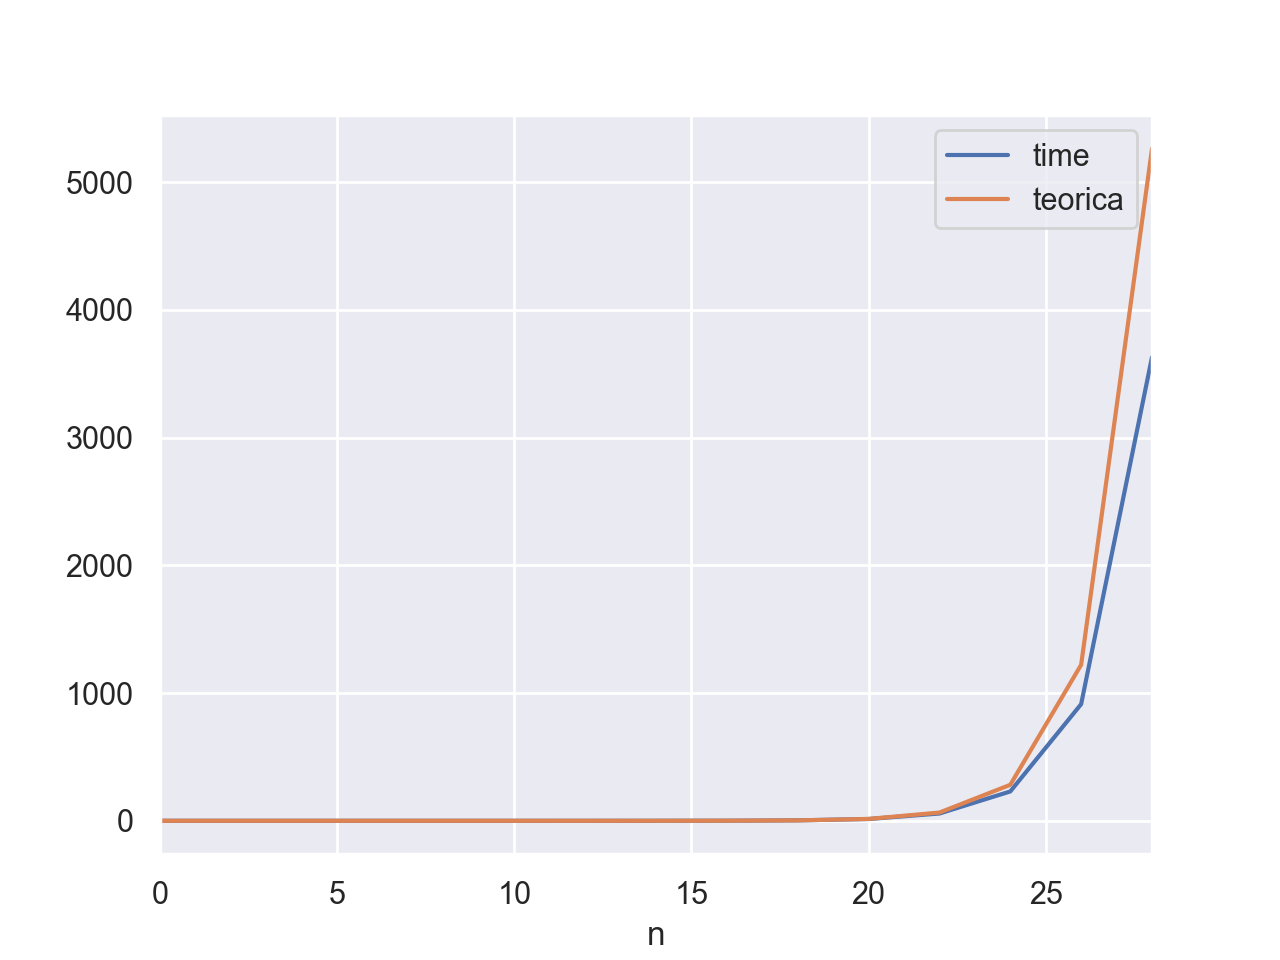
\includegraphics[width=1\linewidth]{img/sinPodas1}
     \caption{Comparación del gráfico de los resultados contra la cota teórica}
   \end{minipage}\hfill
   \begin{minipage}{0.6\textwidth}
     \centering
     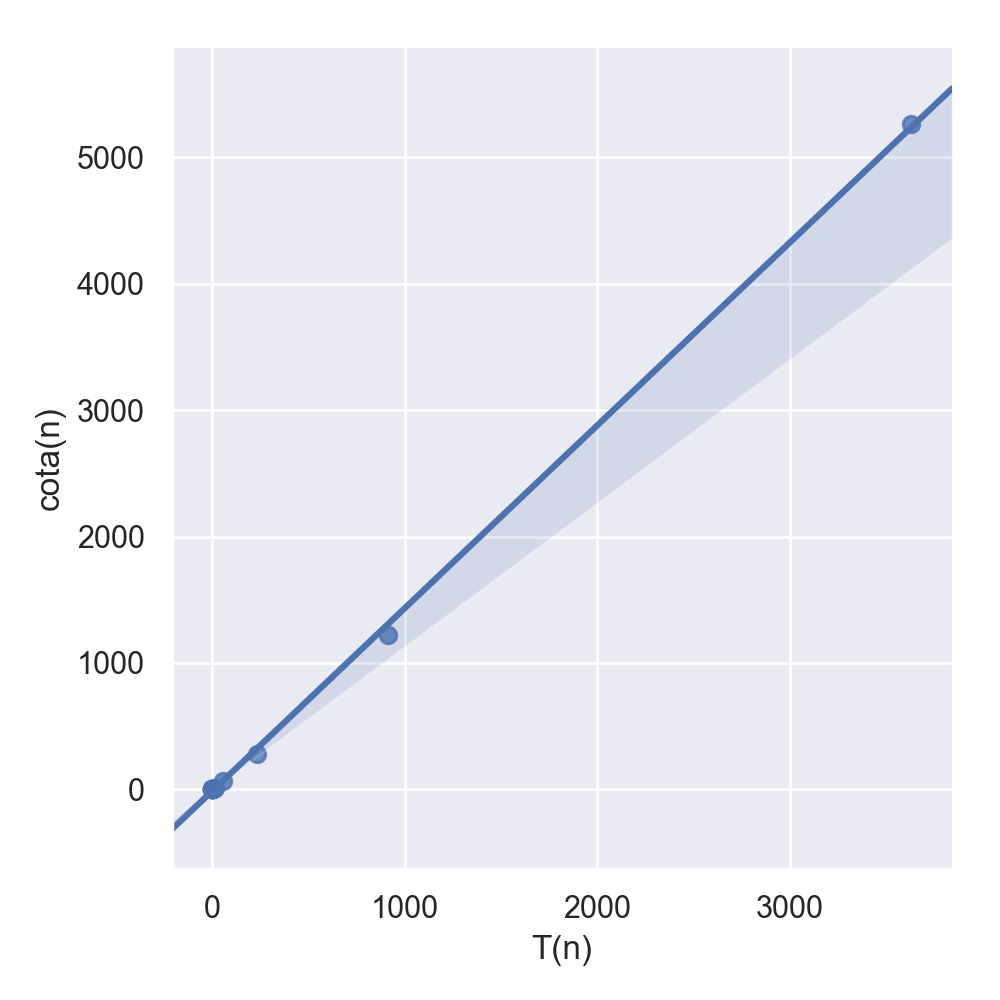
\includegraphics[width=1\linewidth]{img/sinPodas2}
     \caption{Correlación entre algoritmo y cota teórica}
   \end{minipage}
\end{figure}

Como podemos observar en el primer gráfico, podemos observar que la cota teórica tiene un crecimiento un poco más acelerado que nuestros datos. Esto es un resultado que nos sorprende, ya que como vimos antes, la complejidad de éste algoritmo se puede calcular de manera sencilla. Creemos que esta diferencia puede deberse a que no fue posible experimentar demasiados valores de N, dado que el tiempo de ejecución no nos lo permitió.
\newline
Ésta misma diferencia se ve plasmada en el segundo gráfico. En este caso, podemos ver que nuestros datos tienen una correlación positiva con la cota que, aunque es bastante fuerte, no es tan ajustada como por ejemplo en el algoritmo de Meet in the Middle.

\subsection{Experimentación sobre el algoritmo de Meet in the Middle}

En el caso de Meet in the Middle, variamos N en un rango de 0 a 50, y comparamos nuestros resultados con la cota teórica O($n*2^{n/2}$). Los siguientes gráficos muestran nuestros resultados:

\begin{figure}[!htb]
   \begin{minipage}{0.6\textwidth}
     \centering
     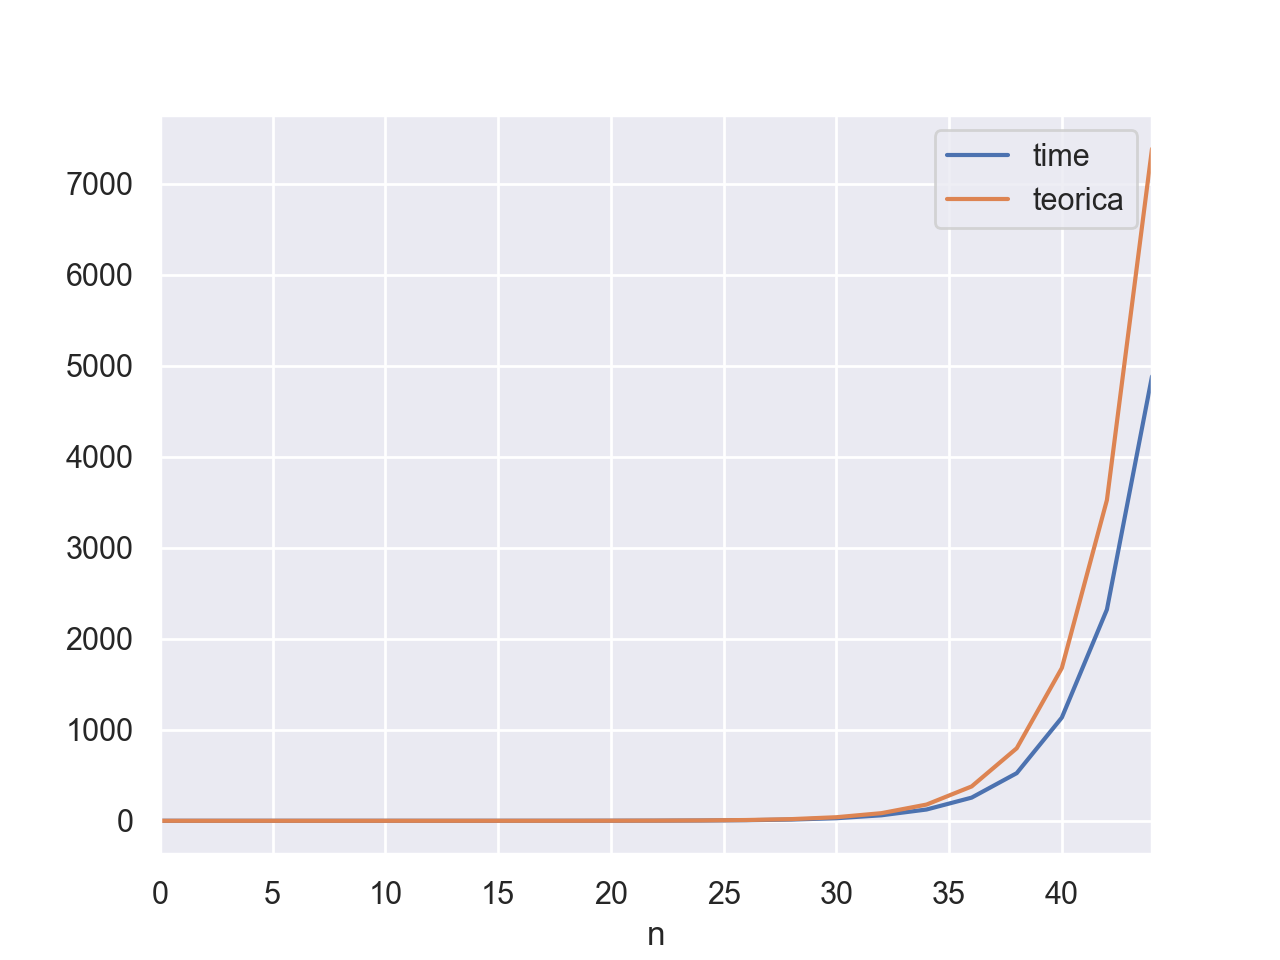
\includegraphics[width=1\linewidth]{img/Middle1}
     \caption{Comparación del gráfico de los resultados contra la cota teórica}
   \end{minipage}\hfill
   \begin{minipage}{0.6\textwidth}
     \centering
     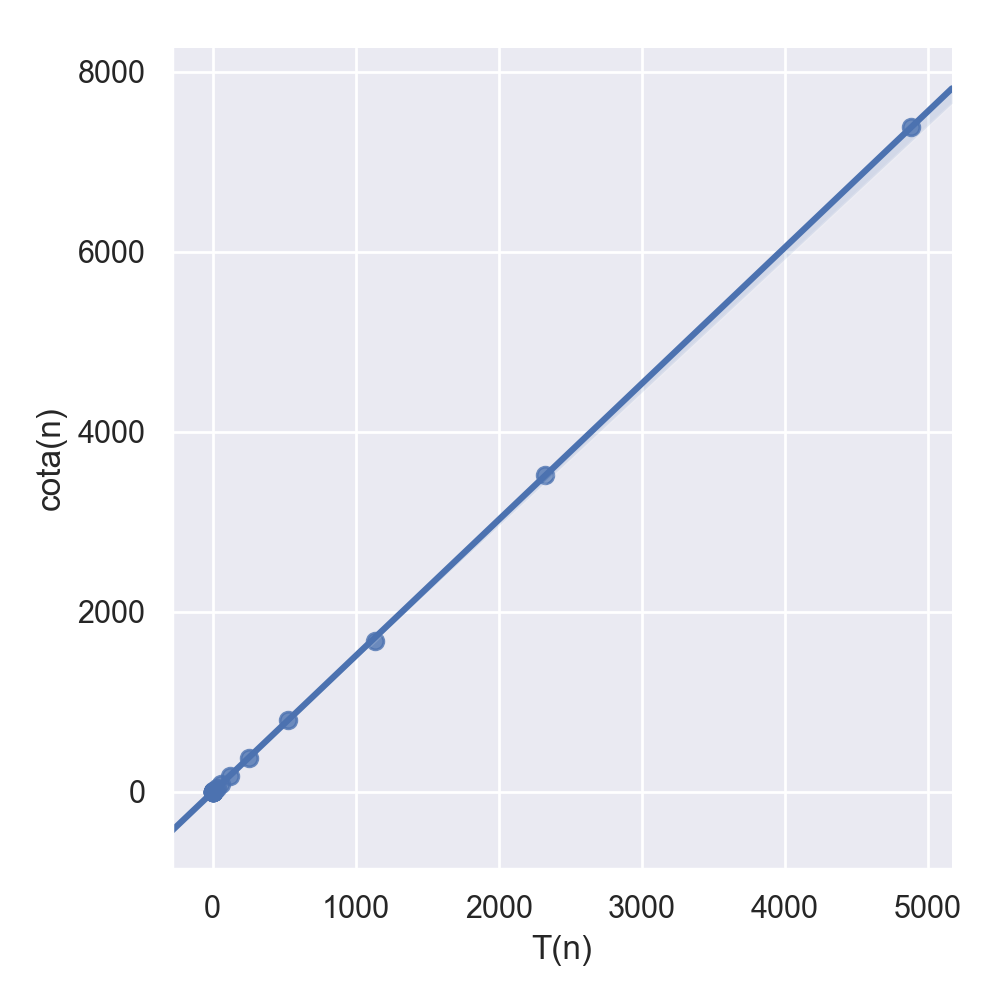
\includegraphics[width=1\linewidth]{img/Middle2}
     \caption{Correlación entre algoritmo y cota teórica}
   \end{minipage}
\end{figure}

Como podemos observar en el primer gráfico, parecería ser que el tiempo de ejecución se ajusta fuertemente a la cota teórica. Ambas funciones parecen tener un crecimiento similar, pero podemos corroborar esto más apropiadamente con el segundo gráfico. Aquí, vemos que nuestros datos tienen una correlación positiva casi perfecta con la cota teórica. La recta de cuadrados mínimos cubre casi perfectamente a nuestros datos.
\label{sec:experimentacion}



\subsection{Experimentación sobre el algoritmo de Backtracking}
Para el algoritmo de backtracking, comenzamos con un análisis del caso en el que no aplicamos ninguna poda. Como vimos en la sección anterior, tenemos una cota teórica de O($n*2^{n}$). Para ver que tan bien se ajusta nuestro algoritmo a ésta cota, generamos nuestros casos de test variando N entre 0 y 30. Veamos los resultados:

\begin{figure}[!htb]
   \begin{minipage}{0.6\textwidth}
     \centering
     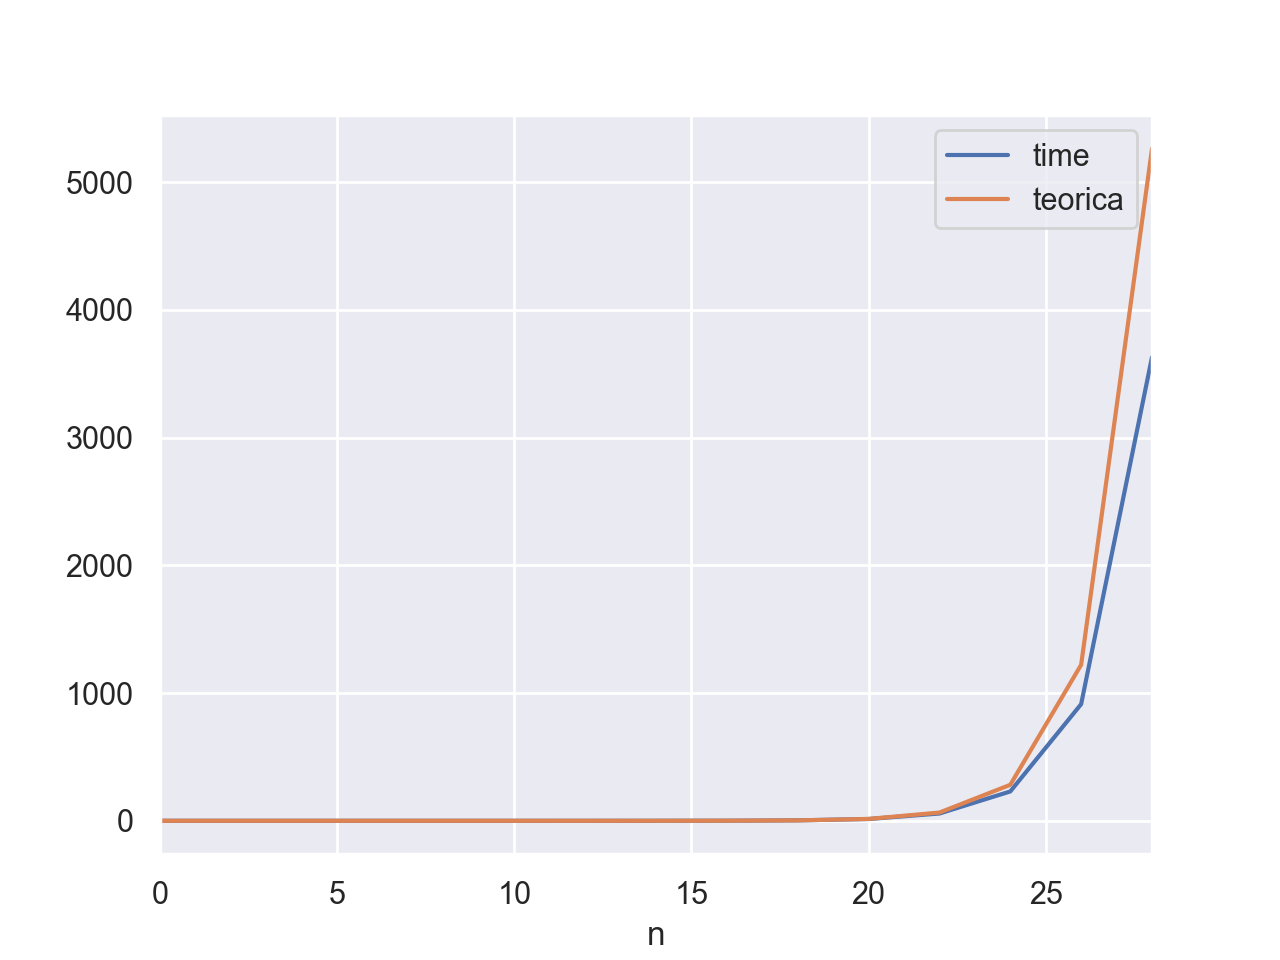
\includegraphics[width=1\linewidth]{img/sinPodas1}
     \caption{Comparación del gráfico de los resultados contra la cota teórica}
   \end{minipage}\hfill
   \begin{minipage}{0.6\textwidth}
     \centering
     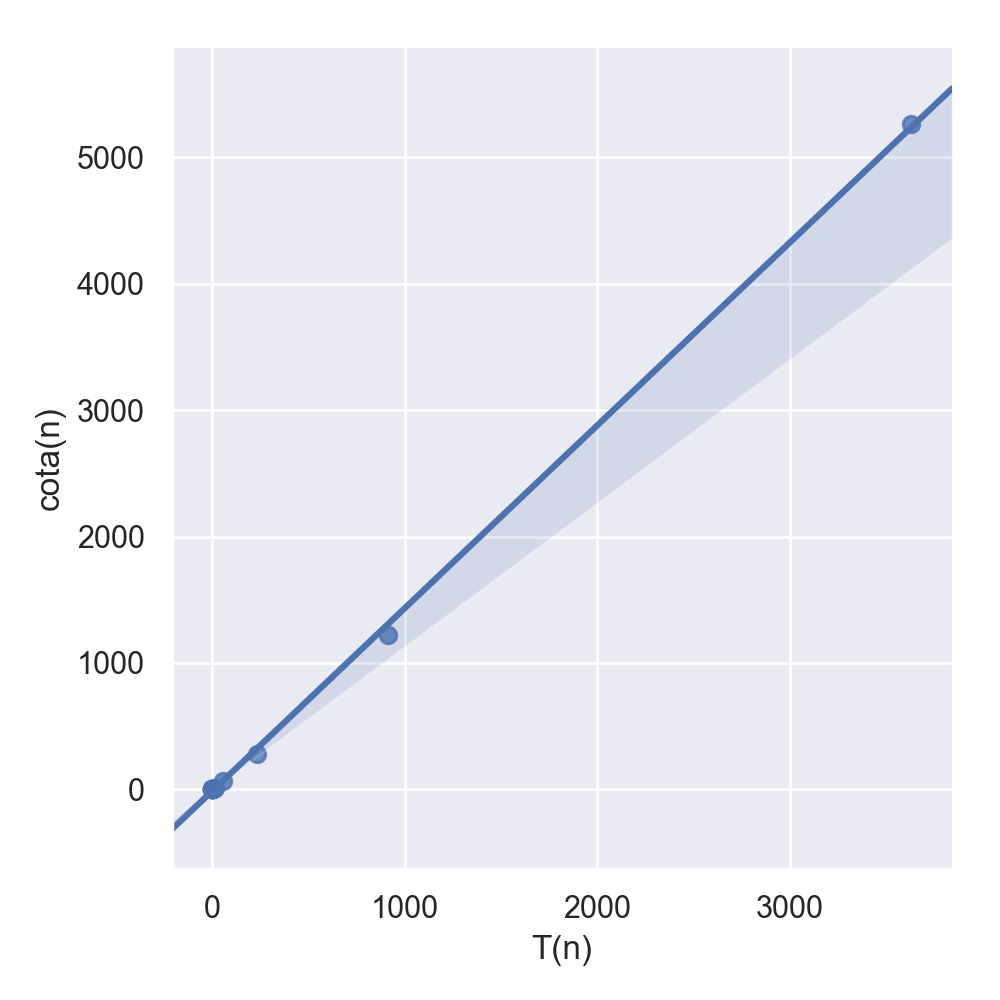
\includegraphics[width=1\linewidth]{img/sinPodas2}
     \caption{Correlación entre algoritmo y cota teórica}
   \end{minipage}
\end{figure}

Como podemos observar en el primer gráfico, podemos observar que la cota teórica tiene un crecimiento un poco más acelerado que nuestros datos. Esto es un resultado que nos sorprende, ya que como vimos antes, la complejidad de éste algoritmo se puede calcular de manera sencilla. Creemos que esta diferencia puede deberse a que no fue posible experimentar demasiados valores de N, dado que el tiempo de ejecución no nos lo permitió.
\newline
Ésta misma diferencia se ve plasmada en el segundo gráfico. En este caso, podemos ver que nuestros datos tienen una correlación positiva con la cota que, aunque es bastante fuerte, no es tan ajustada como por ejemplo en el algoritmo de Meet in the Middle.

\section{Conclusiones}
\label{sec:conclusiones}

Se nos pidió implementar diferentes programas en lenguaje C++ que resuelvan el mismo problema (Problema de la Mochila 1-0) explicado en el enunciado del trabajo practico, mediante diferentes técnicas algorítmicas.
Para la correcta resolución del mismo utilizamos los diferentes paradigmas algorítmicos vistos en clase, y fuimos capaces de aplicar los conceptos teóricos que los distintos métodos proponen al problema practico de obtener el máximo beneficio al tener una mochila de capacidad dada y un conjunto de pedidos distintos, cada uno con un peso y beneficio asociado.


Durante el desarrollo y la resolución del mismo observamos el gran potencial de los distintos métodos para este tipo de problemas. No obstante, pudimos observar como ciertas técnicas tienen una eficiencia temporal notablemente mejor (programación dinámica, backtracking con podas) sobre el resto de las técnicas (fuerza bruta, meet in the middle, etc) que las hace preferibles. Notamos también que aquellos métodos que proveen una mejor eficiencia temporal suelen conllevar una mayor dificultad a la hora de aplicar y codear la solución. Por lo tanto, aparece cierto $trade-off$ entre dificultad a la hora de aplicar la técnica y, la eficiencia del algoritmo final.
Sin embargo, el conocimiento de los distintos paradigmas algorítmicos nos provee de una posible forma de encarar el problema, sin tener en cuenta su complejidad temporal, cuando en principio podríamos no tener una idea solida de como resolver el mismo. De esta manera, el conocimiento de las mismas resulta en una ventaja a la hora de enfrentar nuevos y mas problemas.


\appendix



\end{document}
